\documentclass{article}
\usepackage{color}
\usepackage{graphicx}
\usepackage{amsmath}
\usepackage[margin=0.75in]{geometry}

\begin{document}
\let\thefootnote\relax\footnotetext{Last edited March 14, 2015 by KO}

\section{Methods}

\subsection{Data}
We split the data by year, 1990 and 2010, in which the sodium data was recorded.  We removed Chile from the analysis because there was no life expectancy data for 2010. 36 countries remained.  \\

There was no data on alcohol consumption in Taiwan.  We imputed the missing 2010 sex-specific alcohol consumption for Taiwan using a linear regression of male and female life expectancy, male and female salt consumption, and per capita GDP on sex-specific alcohol consumption in 2010 for all countries. Then we imputed the missing 1990 overall alcohol consumption for Taiwan in the same way, regressing predictors on overall alcohol consumption in 1990 for all countries. \\
 
There was no data for overall alcohol consumption levels in 2010, so we imputed them. A country's population average alcohol consumption was estimated by taking a weighted average of the country's male and female alcohol consumption, weighting by the proportion of males and females in the population.  On the other hand, there was no sex-specific alcohol consumption data for 1990.  For each country, we used the proportion of alcohol consumption in 2010 attributable to males and females to estimate the male and female sex-specific alcohol consumption in 1990, respectively, using the formula

$$\text{Male ETOH in 1990} \approx \text{Overall ETOH in 1990} \times \frac{\text{ Male ETOH in 2010}}{\text{ Imputed overall ETOH in 2010}}$$

\noindent A similar formula applies to females. \\

Finally, we took the difference between 2010 and 1990 for all (numeric) variables and split the data by sex.

\subsection{Statistical analysis}
We tested the hypothesis of association between sodium intake and excess mortality.  In our dataset, ``excess mortality'' is signified by a decrease in life expectancy from 1990 to 2010 beyond what would be expected given the other characteristics of a country.  We measured this by modeling the change in life expectancy using a minimal set of covariates, not including the treatment of interest.  For our dataset, we fit several predictive models (ordinary linear regression, linear regression with polynomial terms, regression trees, bagged regression trees, random forests, boosted trees, and neural networks).  For each type of model, we tuned the parameters by training on bootstrap samples of the data and choosing the tuning parameter that results in the smallest average prediction error.  Finally, from among these tuned models, we chose the model with the smallest mean squared error.  The residuals from the models represent the change in life expectancy not explained by alcohol consumption and per capita GDP. \\

We measured the strength of the association between sodium intake and the residuals from the model using Pearson's correlation. We tested the significance of the association using a permutation test.  Under the null hypothesis of no association, the residuals of the model are exchangeable: if sodium intake has no effect on mortality, then the residuals are equally likely to be paired with any of the sodium measurements.  Under the alternative hypothesis, our model will tend to \textit{overestimate} the increase in life expectancy from 1990 to 2010 in countries where sodium intake increased and to \textit{underestimate} the change in life expectancy in countries where sodium intake decreased. This alternative corresponds to a significant positive correlation between the residuals and change in sodium intake.  


\section{Results}
\subsection{Sodium consumption and life expectancy}
We predicted life expectancy separately for males and females using change in smoking prevalence, change in alcohol consumption, and per capita GDP.  For both males and females, the predictive model with best fit was a random forest.  The correlation for males was $0.003$ (one-sided p-value $0.4835$, two-sided p-value $0.9854$) and the correlation for females was $-0.2640$ (one-sided p-value $0.9382$, two-sided p-value $0.1215$) (Figure~\ref{fig:sodium_excessmortality}). We conclude there is insufficient evidence to reject the null hypothesis that the correlation is $0$.  In fact, the correlation between change in sodium consumption and excess mortality for females is significantly less than $0$.  This means that for females in a particular country, an increase in sodium consumption is associated with a greater change in life expectancy than we would predict given that country's female alcohol consumption, female smoking prevalence, and per capita GDP. \\



\begin{figure}[h]
\centering
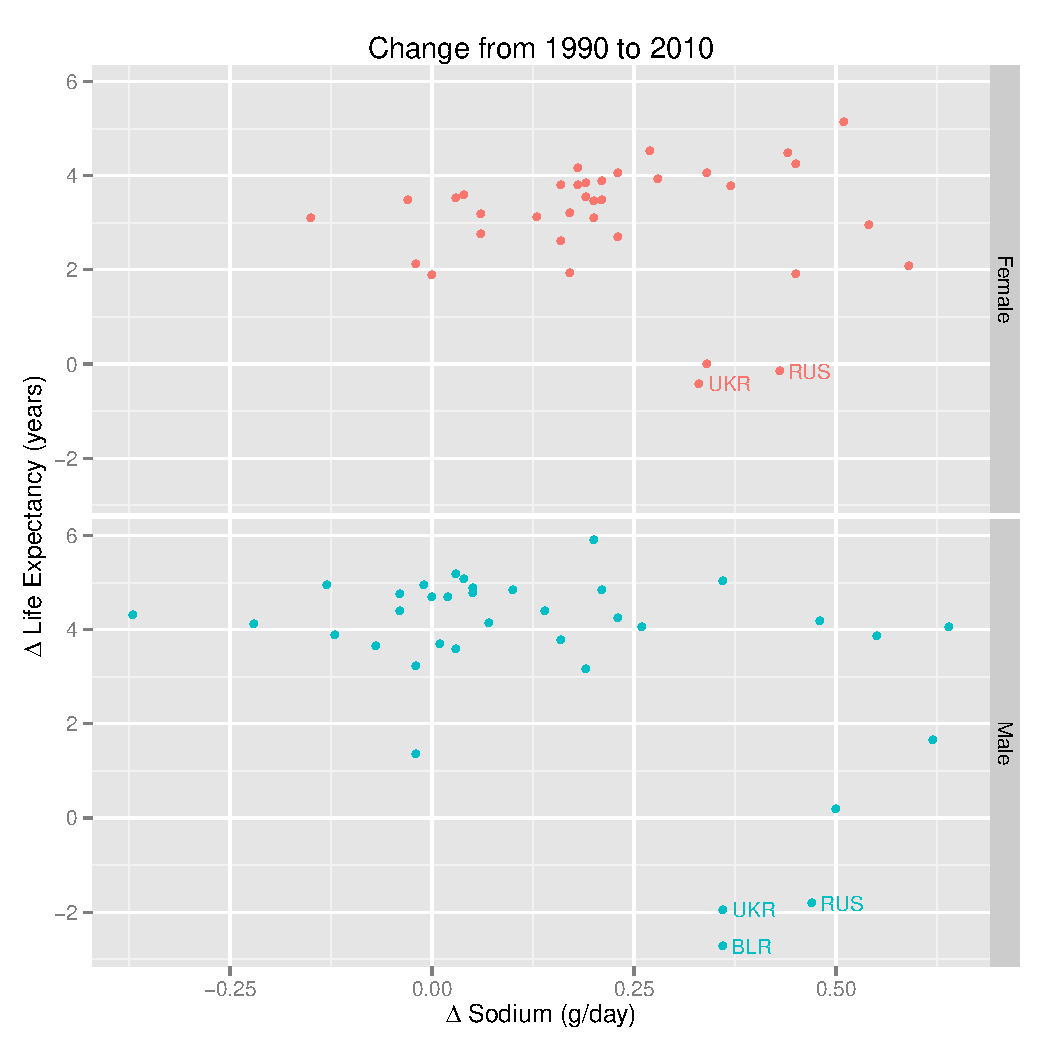
\includegraphics[width = 0.4\textwidth]{sodium_lifeexp.pdf}
\caption{Scatterplot of change in sodium intake against change in life expectancy at age 30 from 1990 to 2010. Even before correcting for the effect of other social and economic factors, there is no obvious association between sodium and life expectancy.}\label{fig:sodium_lifeexp}
\end{figure}[h]

\begin{figure}[h]
\centering
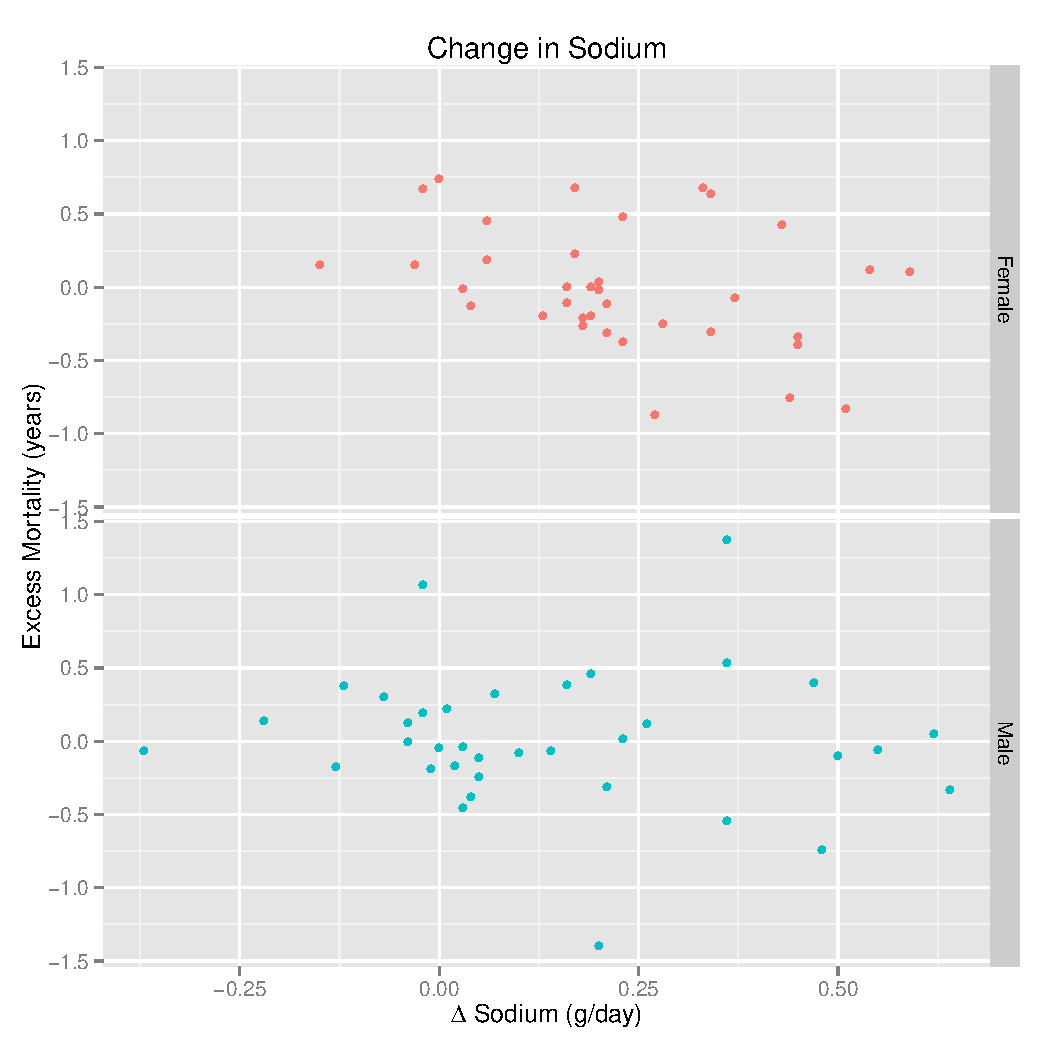
\includegraphics[width = 0.4\textwidth]{sodium_exmort.pdf}
\caption{Scatterplot of change in sodium intake against excess mortality.}\label{fig:sodium_excessmortality}
\end{figure}[h]


\clearpage
\subsection{Smoking prevalence and life expectancy}
We repeated the analysis, switching the roles of sodium and age-standardized prevalence of smoking.  We predicted life expectancy separately for males and females using alcohol consumption and per capita GDP.  As before, the models with best fit for males and females were random forests.  The correlation between excess mortality and change in tobacco use from 1990 to 2010 for males was $0.0663$ (one-sided p-value $0.3489$, two-sided p-value $0.7059$).  The correlation between excess mortality and change in tobacco use from 1990 to 2010 for females was $-0.078$ (one-sided p-value $0.6749$, two-sided p-value $0.6574$).  There is insufficient evidence to reject the null hypothesis that there is no association between change in smoking habits and the change in life expectancy not explained by our prediction model.


\begin{figure}[h]
\centering
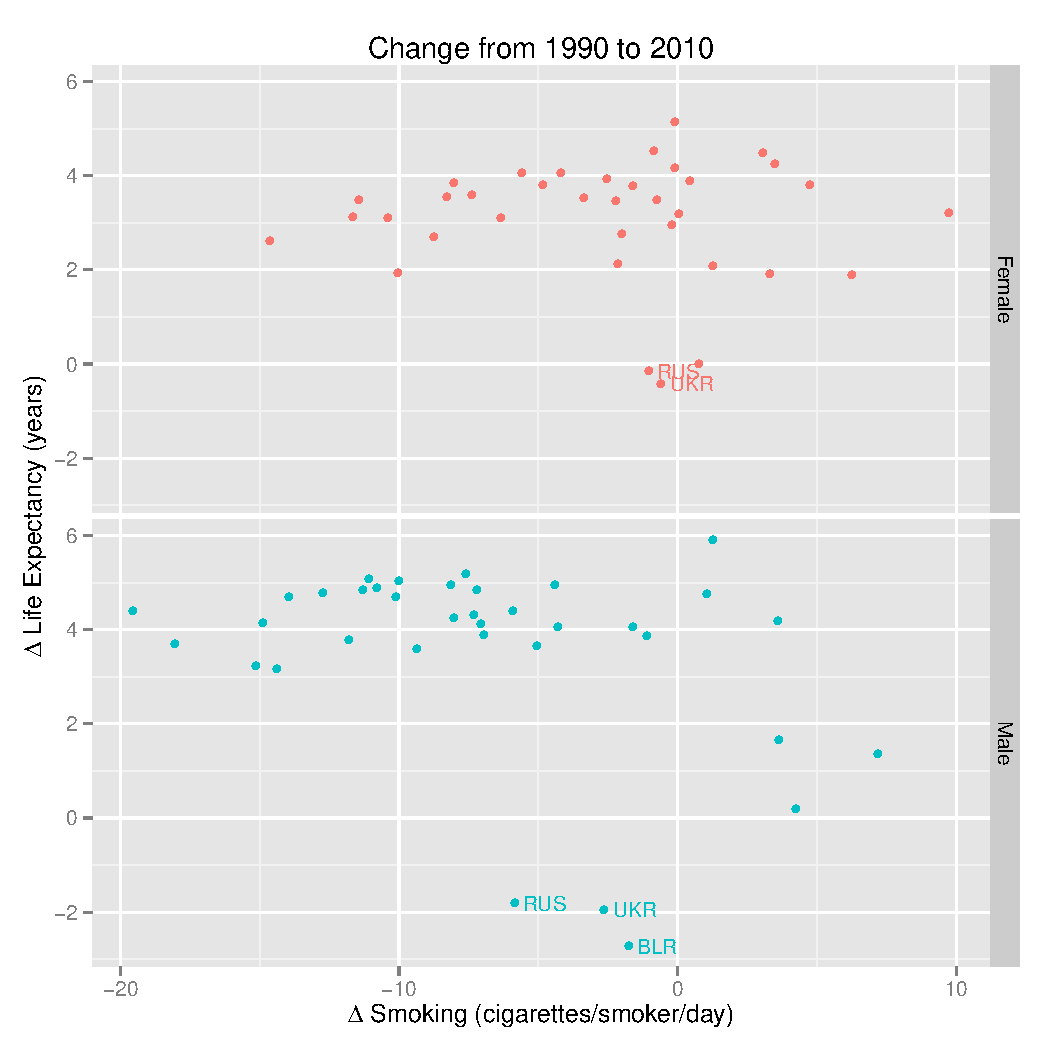
\includegraphics[width = 0.4\textwidth]{smoking_lifeexp.pdf}
\caption{Scatterplot of change in age standardized smoking prevalence against change in life expectancy at age 30 from 1990 to 2010.}\label{fig:smoking_lifeexp}
\end{figure}[h]

\begin{figure}[h]
\centering
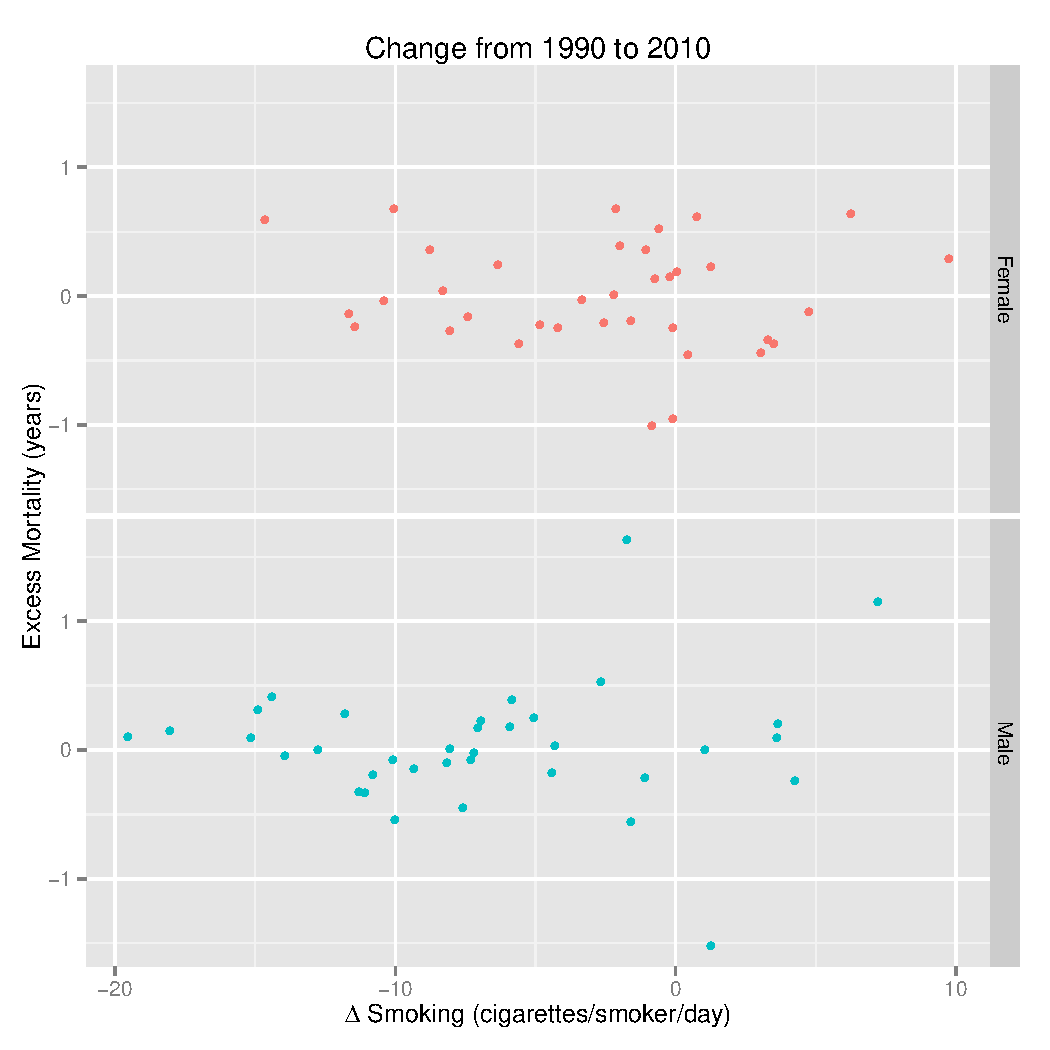
\includegraphics[width = 0.4\textwidth]{smoking_exmort.pdf}
\caption{Scatterplot of change in age standardized smoking prevalence against excess mortality.}\label{fig:smoking_excessmortality}
\end{figure}[h]


\clearpage
\subsection{Cigarettes smoked per capita and life expectancy}
We repeated the analysis using number of cigarettes (in millions) per capita instead of age-standardized prevalence of smoking.  We predicted life expectancy separately for males and females using alcohol consumption and per capita GDP.  As before, the models with best fit for males and females were random forests.  The correlation between excess mortality and change in tobacco use from 1990 to 2010 for males was $0.1922$ (one-sided p-value $0.1285$, two-sided p-value $0.2539$).  The correlation between excess mortality and change in tobacco use from 1990 to 2010 for females was $-0.1204$ (one-sided p-value $0.7589$, two-sided p-value $0.4813$).  There is insufficient evidence to reject the null hypothesis that there is no association between change in smoking habits and the change in life expectancy not explained by our prediction model.


\begin{figure}[h]
\centering
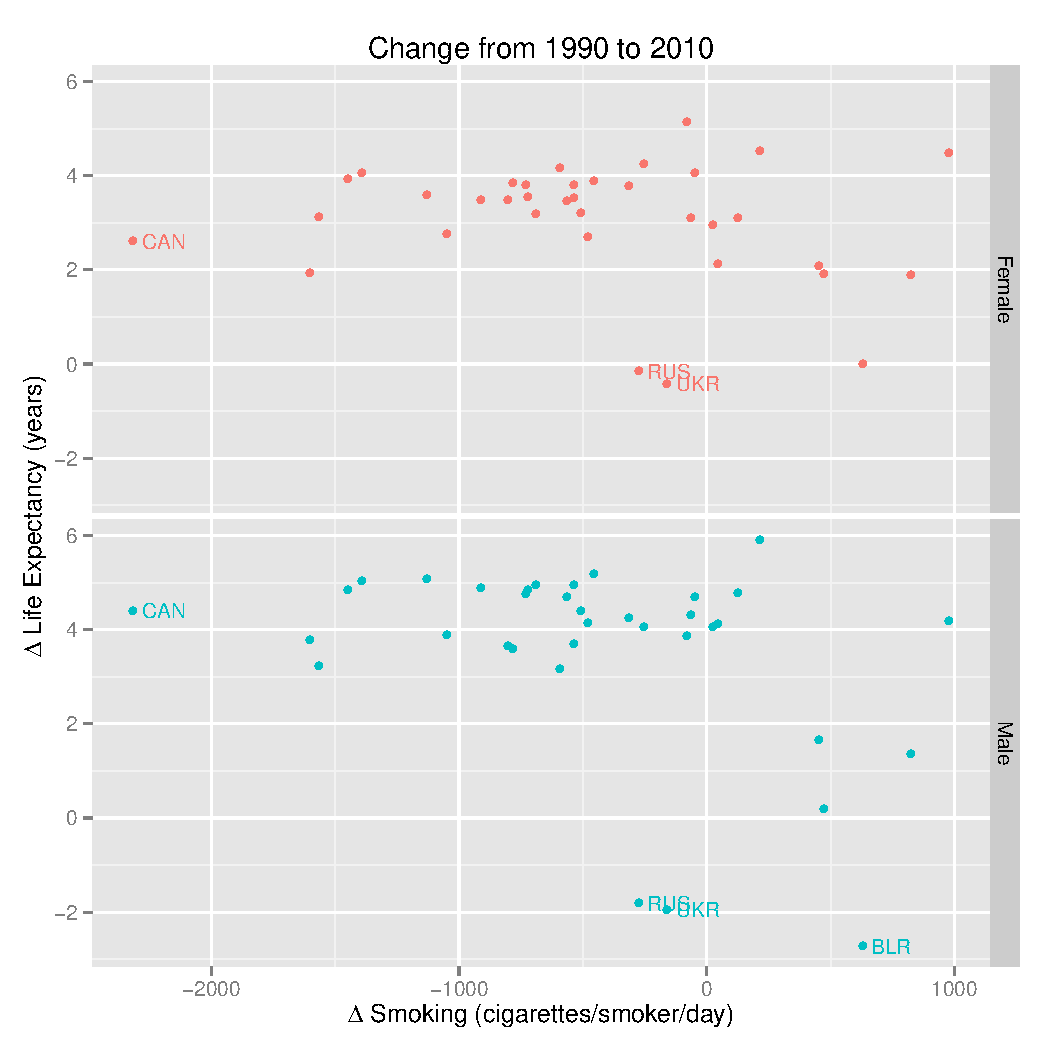
\includegraphics[width = 0.4\textwidth]{smoking_lifeexp2.pdf}
\caption{Scatterplot of change in cigarettes smoked per capita against change in life expectancy at age 30 from 1990 to 2010.}\label{fig:smoking_lifeexp2}
\end{figure}[h]

\begin{figure}[h]
\centering
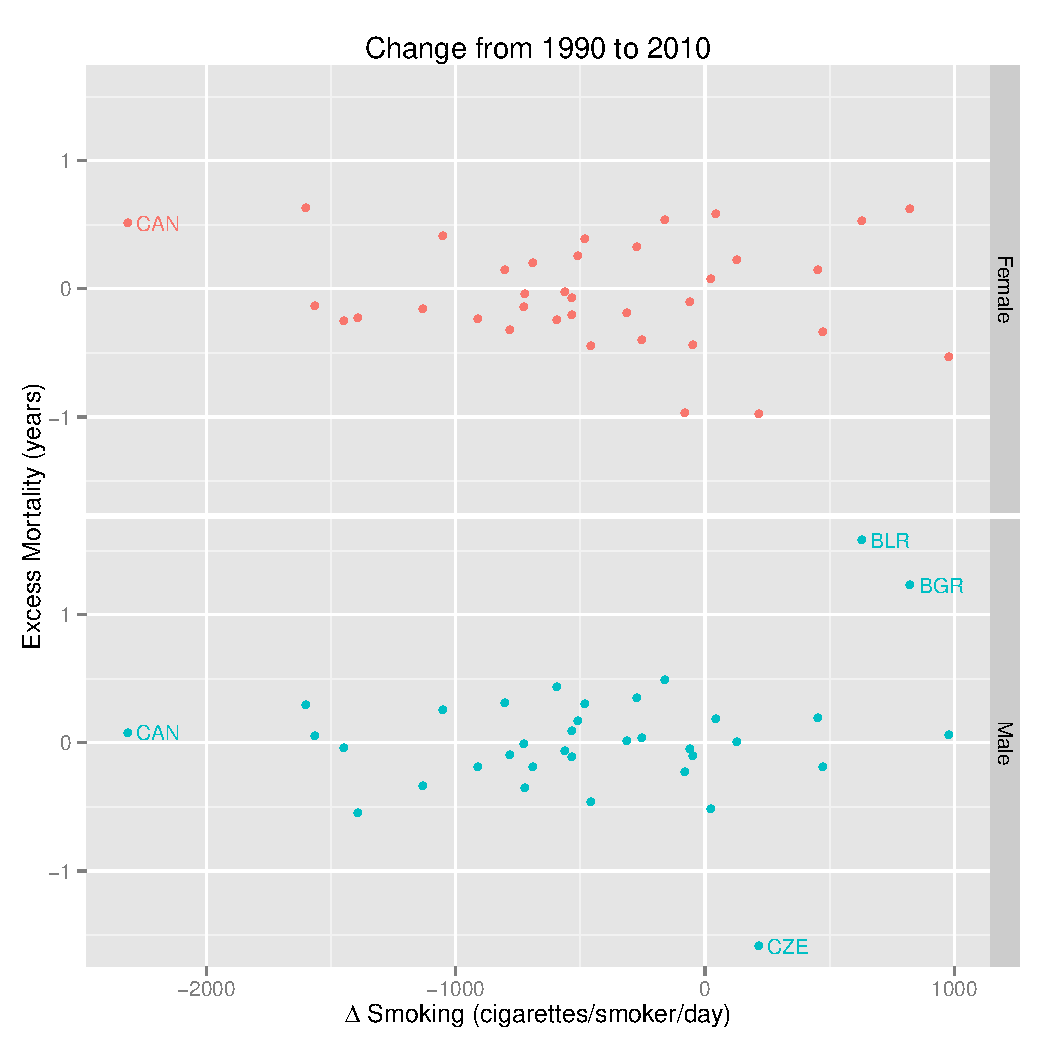
\includegraphics[width = 0.4\textwidth]{smoking_exmort2.pdf}
\caption{Scatterplot of change in cigarettes smoked per capita against excess mortality.}\label{fig:smoking_excessmortality2}
\end{figure}[h]


\subsection{Alcohol and life expectancy}
We repeated the analysis once again, switching the roles of sodium and alcohol consumption, measured in liters of ethanol per year.  We used imputed alcohol consumption data, as described in the first section. We predicted life expectancy separately for males and females using sodium consumption, cigarettes smoked, and per capita GDP.  As before, the models with best fit for males and females were random forests.  The correlation between excess mortality and change in alcohol consumption from 1990 to 2010 for males was $0.4997$ (one-sided p-value $0.0014$, two-sided p-value $0.0021$).  The correlation between excess mortality and change in alcohol consumption from 1990 to 2010 for females was $0.4294$ (one-sided p-value $0.0051$, two-sided p-value $0.0082$).  There is strong evidence in favor of the alternative hypothesis that change in alcohol consumption is positively correlated with a change in mortality greater than what we would predict using only sodium consumption, smoking habits, and per capita GDP.


\begin{figure}[h]
\centering
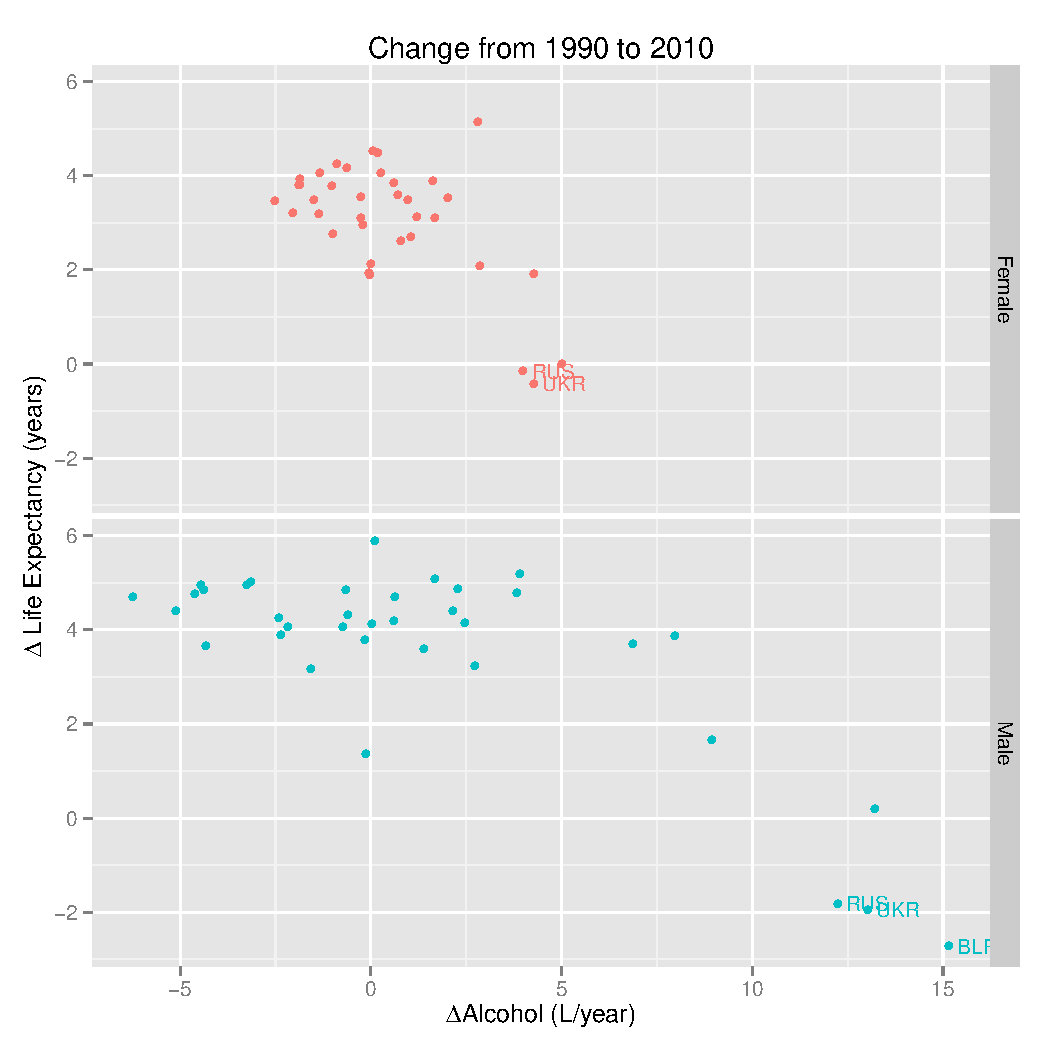
\includegraphics[width = 0.4\textwidth]{etoh_lifeexp.pdf}
\caption{Scatterplot of change in alcohol consumption against change in life expectancy at age 30 from 1990 to 2010.}\label{fig:etoh_lifeexp}
\end{figure}[h]

\begin{figure}[h]
\centering
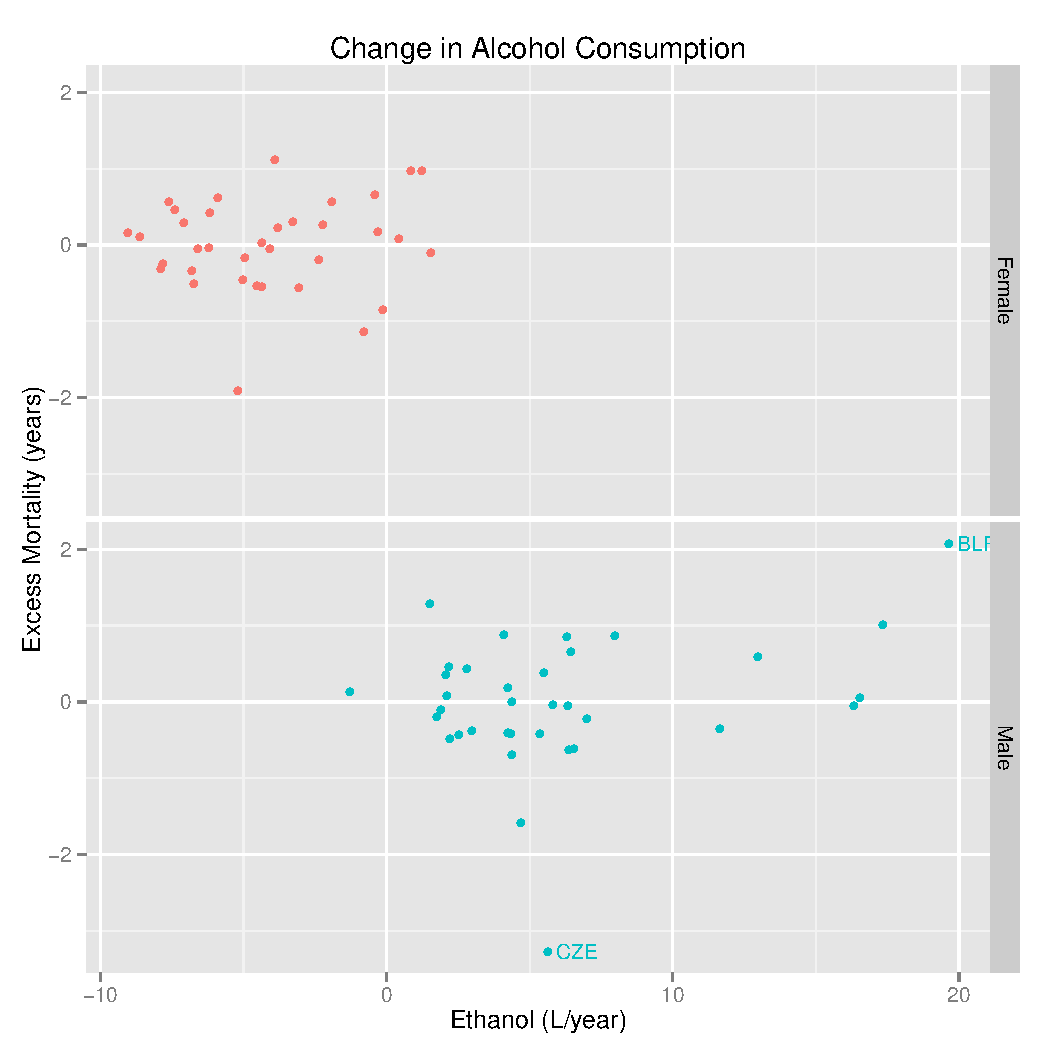
\includegraphics[width = 0.4\textwidth]{etoh_exmort.pdf}
\caption{Scatterplot of change in alcohol consumption against excess mortality.}\label{fig:etoh_excessmortality}
\end{figure}[h]


\clearpage
\section{Discussion}
\subsection{Sensitivity to type of model}
A country's excess mortality is defined as its residual of the model used to predict life expectancy.  One might be concerned about how much the correlation between excess mortality and sodium consumption depends on the choice of model.  We redid the analysis using predictive models other than random forests, including bagged trees, ordinary least squares regression, and boosted trees.  The results from each analysis were consistent with those obtained using random forests. \\

I can flesh out this section further, perhaps report the estimates obtained using several different models, if we think this is interesting/important.  Another thing that might be interesting is to look how the results change if we add more variables (noise) or remove smoking, alcohol, per capita gdp.

\subsection{Absence of correlation between smoking and excess mortality}
It is surprising not to find a correlation between smoking and excess mortality.  To investigate why, we looked at two lines of inquiry.  The first was the issue of sample size.  If we have low power due to a small sample size, then given more data we would find an effect.  To artificially increase the sample size, we subsampled the data and added $N(0, 0.05)$ noise to the covariates, then ran the analysis on this augmented data set.  The augmented data had about $2.5$ times as many observations as the real data. The second issue is confounding between smoking and the covariates used to predict life expectancy.  If one predictor is highly correlated with smoking, then there ought to be very little excess mortality explained by smoking.  We varied the set of predictors of life expectancy and redid the analysis.  \\

Table~\ref{tab:smoking_sensitivity} highlights the issues we face.  First, we notice that the magnitude of the correlation for males is always greater for the subsampled data than for the original data.  This suggests that sample size is in fact an issue.  Second, the confounding between alcohol and smoking affects males and females differently.  This is reflected in the sign of the correlation, which is consistent within gender across each model specification and data set.  \\

Smoking and alcohol consumption are positively correlated for males and negatively correlated for females.  Intuitively, it seems like including alcohol in the model for males should mask the association between smoking and life expectancy.  However, the opposite is true.  We ought to think about what is going on here.

\begin{table}[h]
\begin{center}
\begin{tabular}{l cc|cc }
& Original && Subsampled & \\
\hline\hline
 Model & Correlation & P-value & Correlation & P-value  \\ \hline
 Male, both predictors & 0.0663 & 0.3496 & 0.1721 & 0.0476\\ 
 Female, both predictors & -0.0780 & 0.6745 & -0.0071 & 0.5301\\ \hline
 Male, alcohol only & 0.0260 & 0.4339 & 0.1280 & 0.1173\\ 
 Female, alcohol only & -0.1278 & 0.7704 & -0.0145 & 0.5422\\ \hline
 Male, GDP only & 0.0232 & 0.4443 & 0.0146 & 0.4567\\ 
 Female, GDP only & -0.0581 & 0.6299 & -0.0898 & 0.8063\\ 
\hline
 \end{tabular}
\end{center}
\caption{Correlation and one-sided p-value for smoking prevalence and excess mortality.}
\label{tab:smoking_sensitivity}
\end{table}%



\end{document}